\documentclass[tikz,border=8pt]{standalone}
\usetikzlibrary{arrows.meta,positioning,fit,calc}
\begin{document}
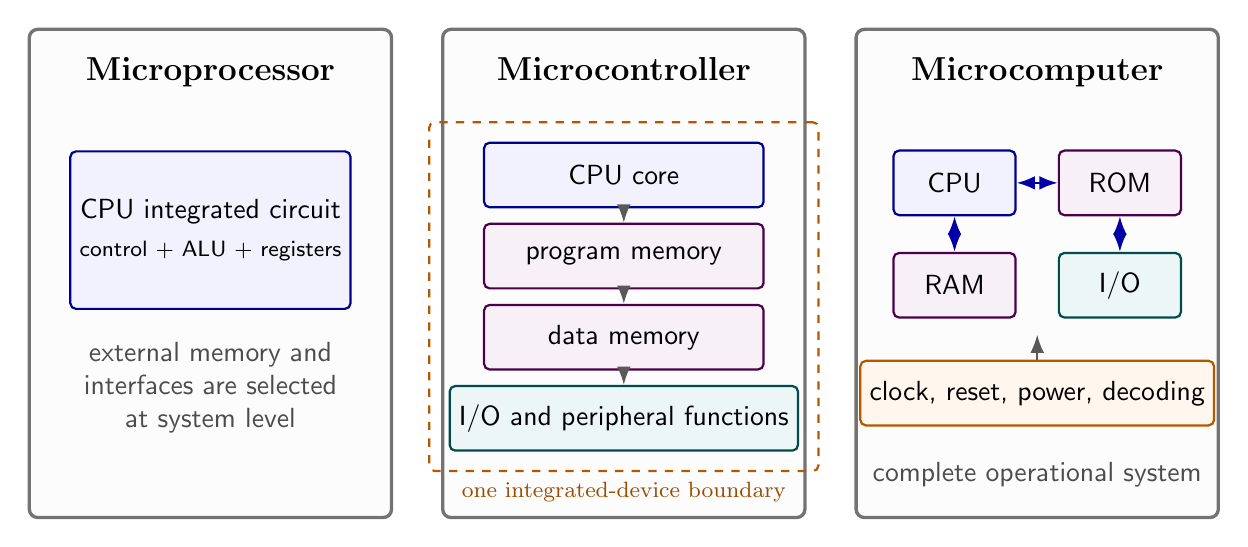
\begin{tikzpicture}[
  font=\sffamily,
  >=Latex,
  panel/.style={draw=black!55,rounded corners=3pt,very thick,minimum width=4.6cm,minimum height=6.2cm,fill=black!1},
  block/.style={draw=blue!55!black,rounded corners=2pt,thick,minimum width=3.55cm,minimum height=.82cm,align=center,fill=blue!5},
  memory/.style={block,draw=violet!60!black,fill=violet!6},
  io/.style={block,draw=teal!60!black,fill=teal!7},
  arrow/.style={->,thick,black!65}
]
  \node[panel] (p1) at (0,0) {};
  \node[font=\bfseries\large,anchor=north] at ([yshift=-.25cm]p1.north) {Microprocessor};
  \node[block,minimum height=2.0cm] (cpu1) at (0,.55) {CPU integrated circuit\\[2pt]\footnotesize control + ALU + registers};
  \node[align=center,text=black!70] at (0,-1.45) {external memory and\\interfaces are selected\\at system level};

  \node[panel] (p2) at (5.25,0) {};
  \node[font=\bfseries\large,anchor=north] at ([yshift=-.25cm]p2.north) {Microcontroller};
  \node[block] (cpu2) at (5.25,1.25) {CPU core};
  \node[memory] (pm2) at (5.25,.22) {program memory};
  \node[memory] (dm2) at (5.25,-.81) {data memory};
  \node[io] (io2) at (5.25,-1.84) {I/O and peripheral functions};
  \node[draw=orange!70!black,dashed,rounded corners=2pt,thick,fit=(cpu2)(pm2)(dm2)(io2),inner sep=7pt,label={[font=\footnotesize,text=orange!60!black]below:one integrated-device boundary}] {};
  \draw[arrow] (cpu2) -- (pm2);
  \draw[arrow] (pm2) -- (dm2);
  \draw[arrow] (dm2) -- (io2);

  \node[panel] (p3) at (10.5,0) {};
  \node[font=\bfseries\large,anchor=north] at ([yshift=-.25cm]p3.north) {Microcomputer};
  \node[block,minimum width=1.55cm] (cpu3) at (9.45,1.15) {CPU};
  \node[memory,minimum width=1.55cm] (rom3) at (11.55,1.15) {ROM};
  \node[memory,minimum width=1.55cm] (ram3) at (9.45,-.15) {RAM};
  \node[io,minimum width=1.55cm] (io3) at (11.55,-.15) {I/O};
  \node[block,draw=orange!70!black,fill=orange!7] (support3) at (10.5,-1.52) {clock, reset, power, decoding};
  \draw[<->,thick,blue!65!black] (cpu3) -- (rom3);
  \draw[<->,thick,blue!65!black] (cpu3) -- (ram3);
  \draw[<->,thick,blue!65!black] (rom3) -- (io3);
  \draw[arrow] (support3.north) -- ++(0,.32);
  \node[align=center,text=black!70] at (10.5,-2.55) {complete operational system};

\end{tikzpicture}
\end{document}
